% debut d'un fichier latex standard
\documentclass[a4paper,12pt,twoside]{article}

\usepackage{lipsum}
\usepackage{empheq}

% pour l'inclusion de figures en eps,pdf,jpg
\usepackage{graphicx}
\usepackage{subcaption}
\usepackage{wrapfig}
% quelques symboles mathematiques en plus
\usepackage{amsmath}
\usepackage{amsthm} % Pour les preuves
% le tout en langue francaise
%\usepackage[french]{babel}
% on peut ecrire directement les caracteres avec l'accent
% a utiliser sur Linux/Windows
\usepackage[utf8]{inputenc}
\usepackage[T1]{fontenc}
% a utiliser sur le Mac
%\usepackage[applemac]{inputenc}
% pour l'inclusion de links dans le document
\usepackage[colorlinks,bookmarks=false,linkcolor=blue,urlcolor=blue]{hyperref}
\usepackage{siunitx}
% pour les degrés
\usepackage{textcomp}
\paperheight=297mm
\paperwidth=210mm

\setlength{\textheight}{235mm}
\setlength{\topmargin}{-1.2cm} % pour centrer la page verticalement
%\setlength{\footskip}{5mm}
\setlength{\textwidth}{15cm}
\setlength{\oddsidemargin}{0.56cm}
\setlength{\evensidemargin}{0.56cm}

\pagestyle{plain}

% quelques abreviations utiles
\def \be {\begin{equation}}
\def \ee {\end{equation}}
\def \dd  {{\rm d}}

\newcommand{\mail}[1]{{\href{mailto:#1}{#1}}}
\newcommand{\ftplink}[1]{{\href{ftp://#1}{#1}}}

\newcommand{\illabel}[1]{ ~ \refstepcounter{equation}(\theequation)\label{#1}} % Ecrit une équation dans le texte, numérotés.
\newcommand{\mbf}[1]{\mathbf{#1}} % bold font in math
\newcommand{\grad}[1]{\nabla#1}
\newcommand{\Div}[1]{\nabla\cdot\mathbf{#1}}
\newcommand{\rot}[1]{\nable\cross\mathbf{#1}}
\newcommand{\bracket}[1]{\left(#1\right)}
\newcommand{\sqbracket}[1]{\left[#1\right]}
\newcommand{\lapl}[1]{\Delta#1}

%
% latex SqueletteRapport.tex      % compile la source LaTeX
% xdvi SqueletteRapport.dvi &     % visualise le resultat
% dvips -t a4 -o SqueletteRapport.ps SqueletteRapport % produit un PostScript
% ps2pdf SqueletteRapport.ps      % convertit en pdf

% pdflatex SqueletteRapport.pdf    % compile et produit un pdf
% \message{================> TAILLE DE LA POLICE EN CM \printinunitsof{cm}\prntlen{\textwidth}}

% ======= Le document commence ici ======

\begin{document}
% Le titre, l'auteur et la date
\title{Wave equation in an inhomogeneous environment\\{\normalsize Normal modes and propagation of the wave of a tsunami}\\{\small Physique Numérique I}\\{\small Rapport 7}}
\date{\today}
\author{Delphine Martres and Damien Korber\\{\small \mail{delphine.martres@epfl.ch} and \mail{damien.korber@epfl.ch}}}

\maketitle
\tableofcontents % Table des matieres


% Quelques options pour les espacements entre lignes, l'identation
% des nouveaux paragraphes, et l'espacement entre paragraphes
\baselineskip=16pt
\parindent=15pt
\parskip=5pt
\newpage

%%%% ON COMMENCE A ECRIRE D'ICI

%===============================================================================
%=============================== INTRODUCTION ==================================
%===============================================================================
\section{Introduction}
  This report will focus on the study of the behaviour of waves in an unidimensional environment.
  These waves will be governed by equations \eqref{eq:ondes-ABC}.

  \begin{align}
    \begin{split}
      \text{Equation A: }&~\frac{\partial^2f}{\partial t^2}=u^2\frac{\partial^2f}{\partial x^2}\\
      \text{Equation B: }&~\frac{\partial^2f}{\partial t^2}=\frac{\partial}{\partial x}\bracket{u^2\frac{\partial f}{\partial x}}\\
      \text{Equation C: }&~\frac{\partial^2f}{\partial t^2}=\frac{\partial^2}{\partial x^2}\bracket{u^2f}
    \end{split}
    \label{eq:ondes-ABC}
  \end{align}

  The domain considered is $x\in\left[0,L\right]$ with different border condition depending on the situation.
  The initial condition is given by $f(x,t=0)=0~\forall x$.




%===============================================================================
%=========================== IMPLEMENTATION ====================================
%===============================================================================
\section{Implementation}
  \subsection{Discretization of the waves equations}

  To discretize equations \eqref{eq:ondes-ABC}, an explicit 3-levels numerical method will be used.
  This means that for any function $g(x)$ twice-differentiable, we get equation \eqref{eq:3-levels-method}.

  \begin{equation}
    \frac{\partial g}{\partial x}(x_i)\approx\frac{g(x_{i+1}) - g(x_{i-1})}{2h}~\text{ and }~\frac{\partial^2 g}{\partial x^2}(x_i)\approx\frac{g(x_{i+1}) - 2g(x_i) + g(x_{i-1})}{h^2}
    \label{eq:3-levels-method}
  \end{equation}

  with $h=x_{i+1} - x_i$.
  Thus, the resulting discretization of the waves equations gives equations \eqref{eq:onde-A-disc}, \eqref{eq:onde-B-disc} and \eqref{eq:onde-C-disc}.
  Note that $f_i^n \equiv f(x_i, t_n)$ and $u_i \equiv u(x_i)$.

  \begin{align}
    \intertext{Equation A:}
    \Aboxed{f^{n+1}_i &= 2f^n_i - f^{n-1}_i + \bracket{\frac{\Delta t}{\Delta x}}^2u^2_i\sqbracket{f^n_{i+1} - 2f^n_i + f^n_{i-1}}}\label{eq:onde-A-disc}
    \intertext{Equation B:}
    \Aboxed{f^{n+1}_i &= 2f^n_i - f^{n-1}_i + \bracket{\frac{\Delta t}{\Delta x}}^2u^2_i\sqbracket{f^n_{i+1} - 2f^n_i + f^n_{i-1}} + \bracket{\frac{\Delta t}{\Delta x}}^2\frac{u_i}{2}(u_{i+1}-u_{i-1})(f^n_{i+1}-f^n_{i-1})}\label{eq:onde-B-disc}
    \intertext{Equation C:}
    \Aboxed{f^{n+1}_i &= 2f^n_i - f^{n-1}_i + \bracket{\frac{\Delta t}{\Delta x}}^2\sqbracket{u^2_{i+1}f^n_{i+1} - 2u^2_if^n_i + u^2_{i-1}f^n_{i-1}}} \label{eq:onde-C-disc}
  \end{align}

  \subsection{Border conditions}
    Multiple border conditions are given for this exercice.
    Furthermore, both side must be separated.
    Note that $u(x) \geq 0~\forall x$ and $f_i^n \equiv f(x_i, t_n)$ and $u_i \equiv u(x_i)$.

    \subsubsection{Left border}
      \paragraph{Fixed.}
        The left fixed condition is simply given by $\boxed{f^{n+1}_0 = f^n_0}$.
      \paragraph{Free.}
      %TODO : À remplir
      \paragraph{Harmonic.}
      %TODO : À remplir
      \paragraph{Exit.}
        \begin{align}
          \intertext{For the left exit, $f$ is given by a strictly backward wave.}
          f(x,t) &= G(x+ut)~\forall x~\forall t
          \intertext{Thus:}
          \frac{\partial f}{\partial t}(x_L, t) &= uG' = u(x_L)\frac{\partial f}{\partial x}(x_L,t) \forall t
          \intertext{By using a forward finite difference for both $x$ and $t$:}
          \frac{f_0^{n+1} - f_0^{n}}{\Delta t} &= u_0\frac{f_1^n - f_0^n}{\Delta x}
          \intertext{Which leads to the left exit border condition.}
          \Aboxed{ f_0^{n+1} &= u_0\frac{\Delta t}{\Delta x}\sqbracket{f_1^n - f_0^n} + f_0^n}\label{eq:left-exit}
        \end{align}

    \subsubsection{Right border}
      \paragraph{Fixed.}
      The right fixed condition is simply given by $\boxed{f^{n+1}_{N} = f^n_N}$. %TODO : C'est juste ça ?
      \paragraph{Free.}
      %TODO : À remplir
      \paragraph{Harmonic.}
      %TODO : À remplir
      \paragraph{Exit.}
      \begin{align}
        \intertext{For the right exit, $f$ is given by a strictly forward wave.}
        f(x,t) &= F(x-ut)~\forall x~\forall t
        \intertext{Thus:}
        \frac{\partial f}{\partial t}(x_R, t) &= -uF' = -u(x_R)\frac{\partial f}{\partial x}(x_R,t) \forall t
        \intertext{By using a forward finite difference for $t$ and a backward finite difference for $x$:}
        \frac{f_N^{n+1} - f_N^{n}}{\Delta t} &= -u_N\frac{f_N^n - f_{N-1}^n}{\Delta x}
        \intertext{Which leads to the right exit border condition.}
        \Aboxed{ f_N^{n+1} &= -u_N\frac{\Delta t}{\Delta x}\sqbracket{f_N^n - f_{N-1}^n} + f_N^n}\label{eq:left-exit}
      \end{align}

    %TODO : À remplir


  \subsection{Energy of the wave}
    The energy of a wave over a domain $x\in\left[0, L\right]$ is given by equation \eqref{eq:energie-continue}.

    \begin{equation}
      E(t) = \int_0^L f^2(x,t)dx
      \label{eq:energie-continue}
    \end{equation}

    An estimation of the integral of any integrable function $g$ can be found using the trapezoidal rule, which is given by equation \eqref{eq:trapeze-rule}.

    \begin{equation}
      \int_a^b g(x)dx \approx h\sum_{i=1}^N\bracket{\frac{g(x_i) + g(x_{i+1})}{2}}
      \label{eq:trapeze-rule}
    \end{equation}

    with $h = x_{i+1} - x_i$.
    Thus, the energy is given by equation \eqref{eq:energie-discret}.

    \begin{equation}
      \boxed{E(t) = (\Delta x)\sum_{k=0}^{N-2}\frac{f^2(x_k) + f^2(x_{k+1})}{2}}\\
      \label{eq:energie-discret}
    \end{equation}

\section{Constant propagation speed}
In this section, $u(x)=const=6$ (which implies equations \eqref{eq:ondes-ABC} are equal) m/s and $L=20$ m.

\subsection{Border reflection}
The left border condition is $f(0,t)=A\sin(\omega t)$ with $A=1$ m and $\omega=5$ rad/s.

\begin{figure}[h]
 \begin{subfigure}{0.5\textwidth}
  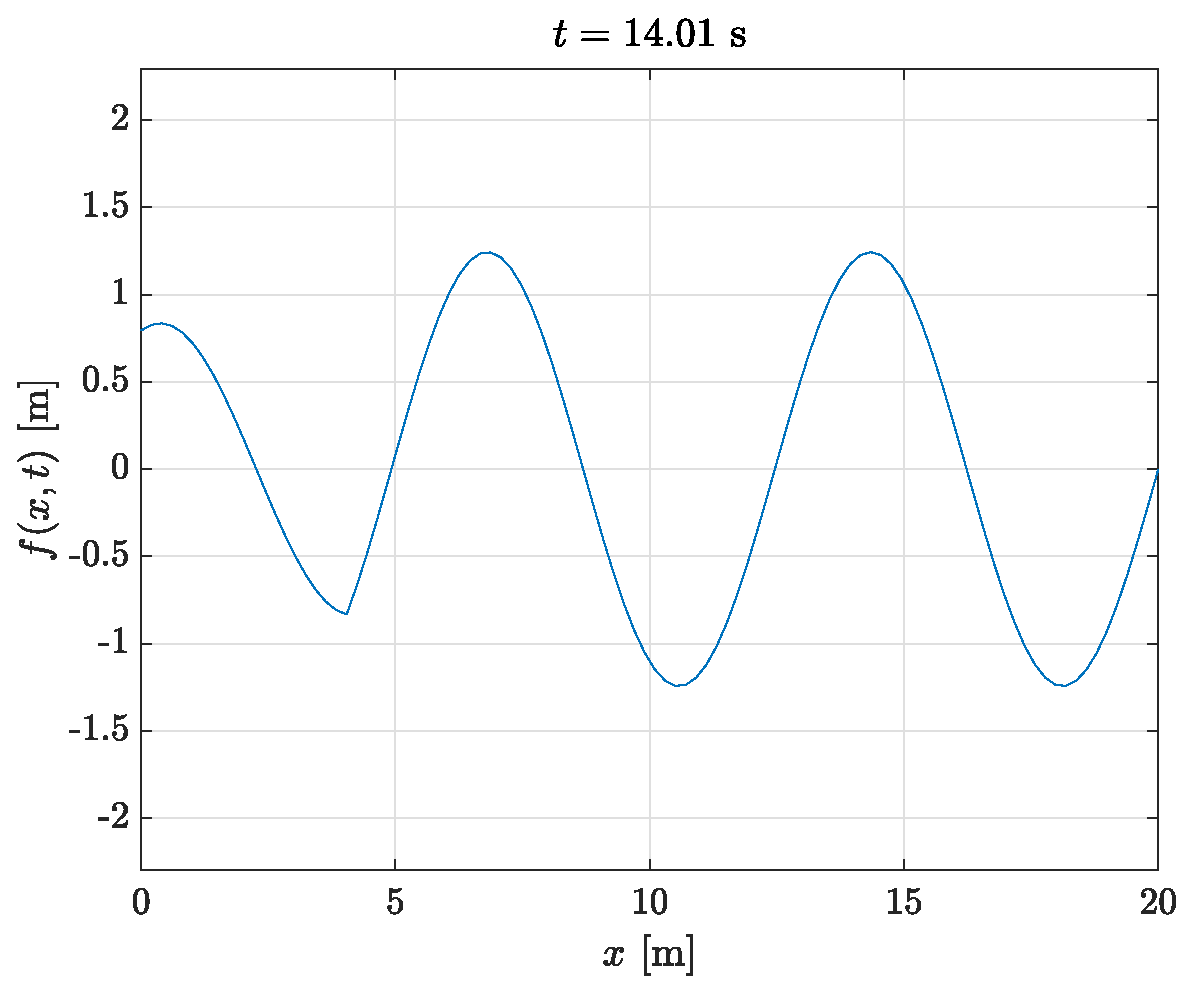
\includegraphics[width=\textwidth]{graphs/ex1ffixe.eps}
 \end{subfigure}
 ~
 \begin{subfigure}{0.55\textwidth}
  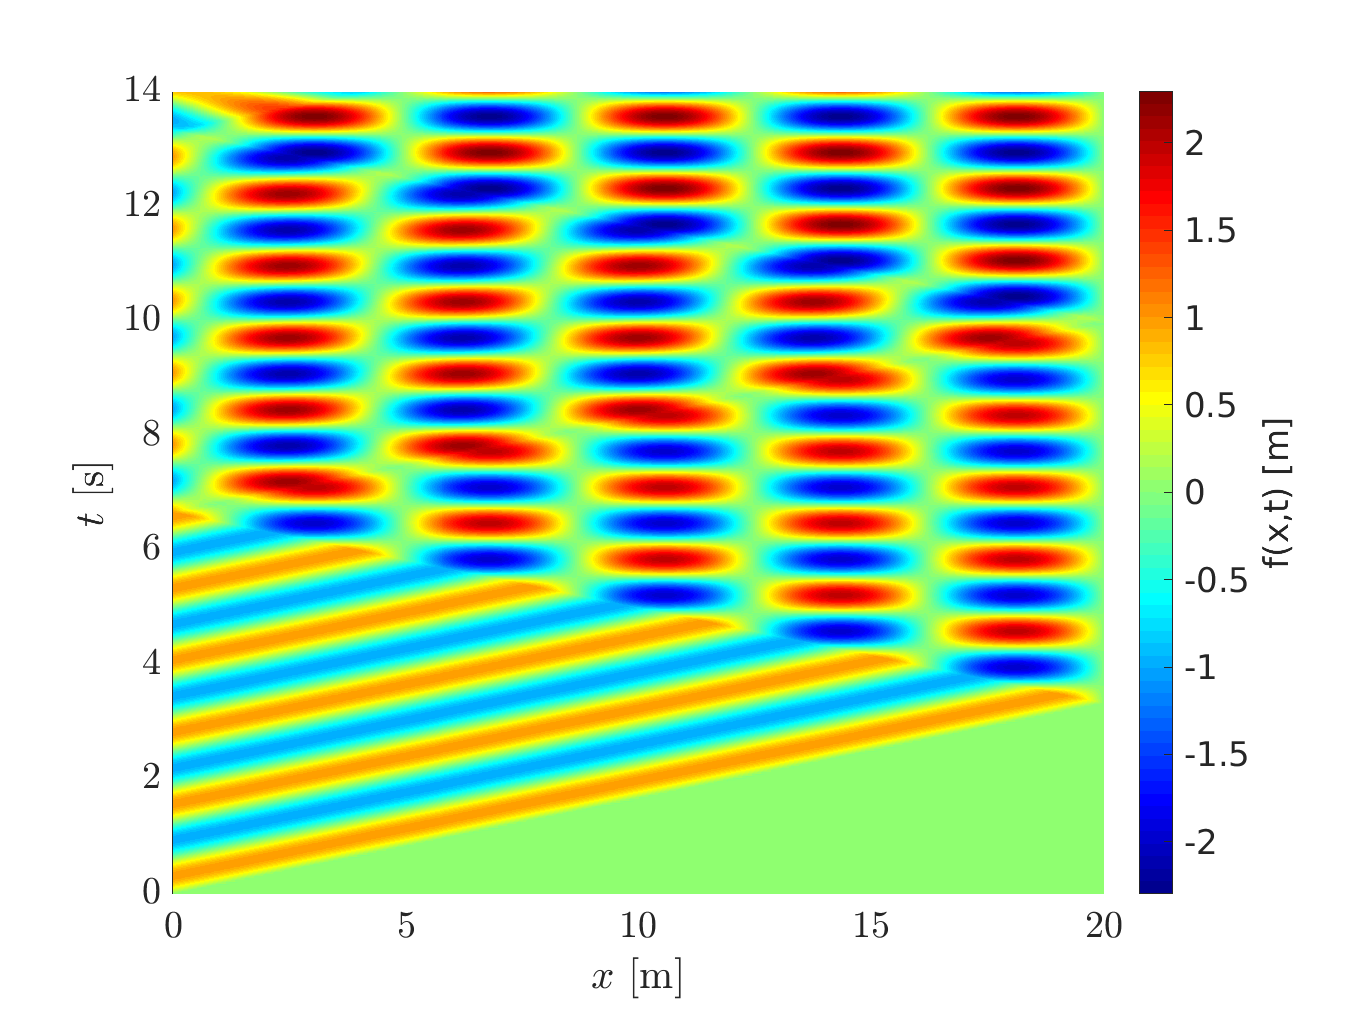
\includegraphics[width=\textwidth]{graphs/ex1xtfixe.eps}
 \end{subfigure}\
 
 \centering
 \begin{subfigure}{0.5\textwidth}
  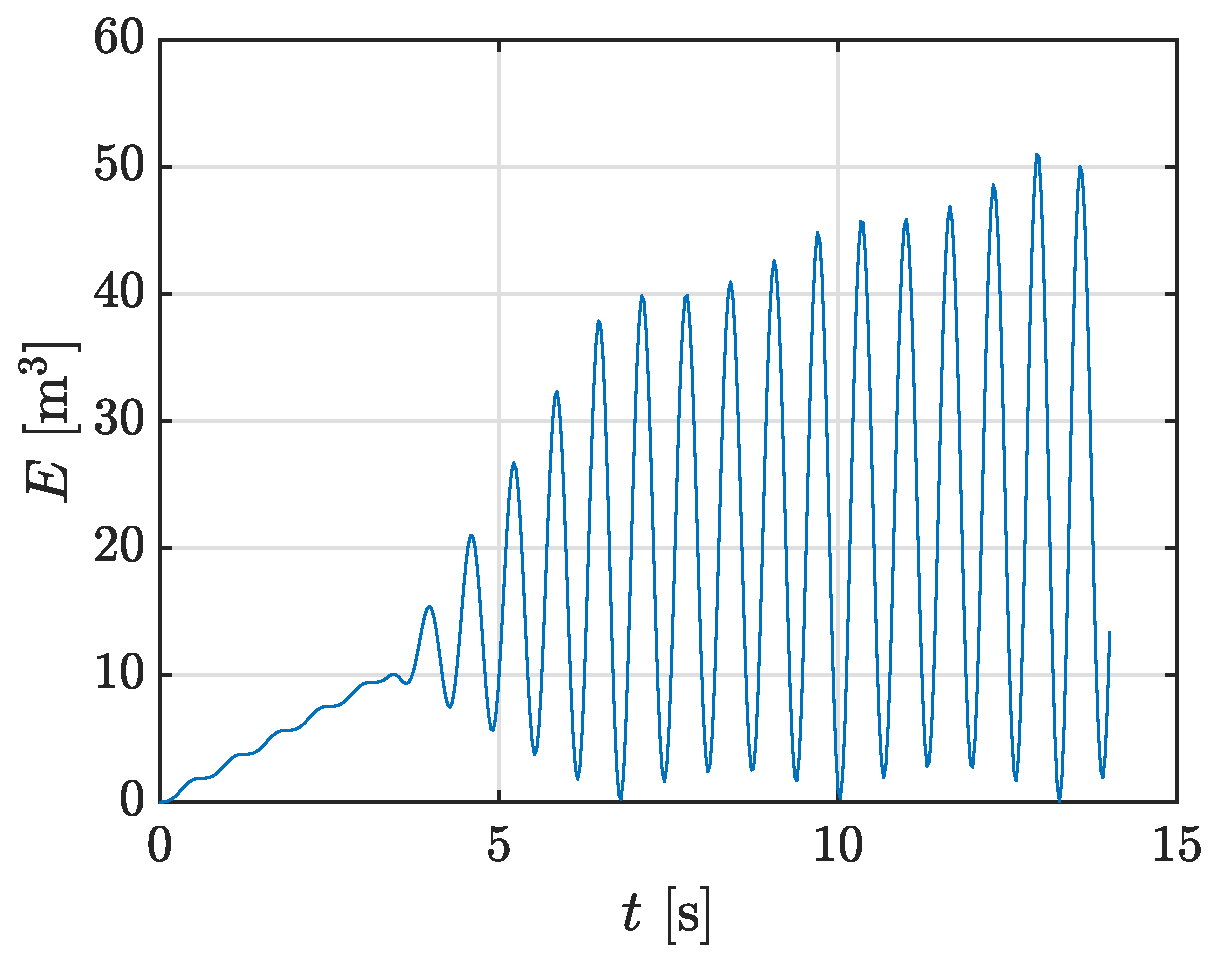
\includegraphics[width=\textwidth]{graphs/ex1Efixe.eps}
 \end{subfigure}

 \caption{Illustration of the border reflection for a the fixed right border condition}
 \label{fig:ex1fix}
\end{figure}



\begin{figure}[h]
 \begin{subfigure}{0.5\textwidth}
  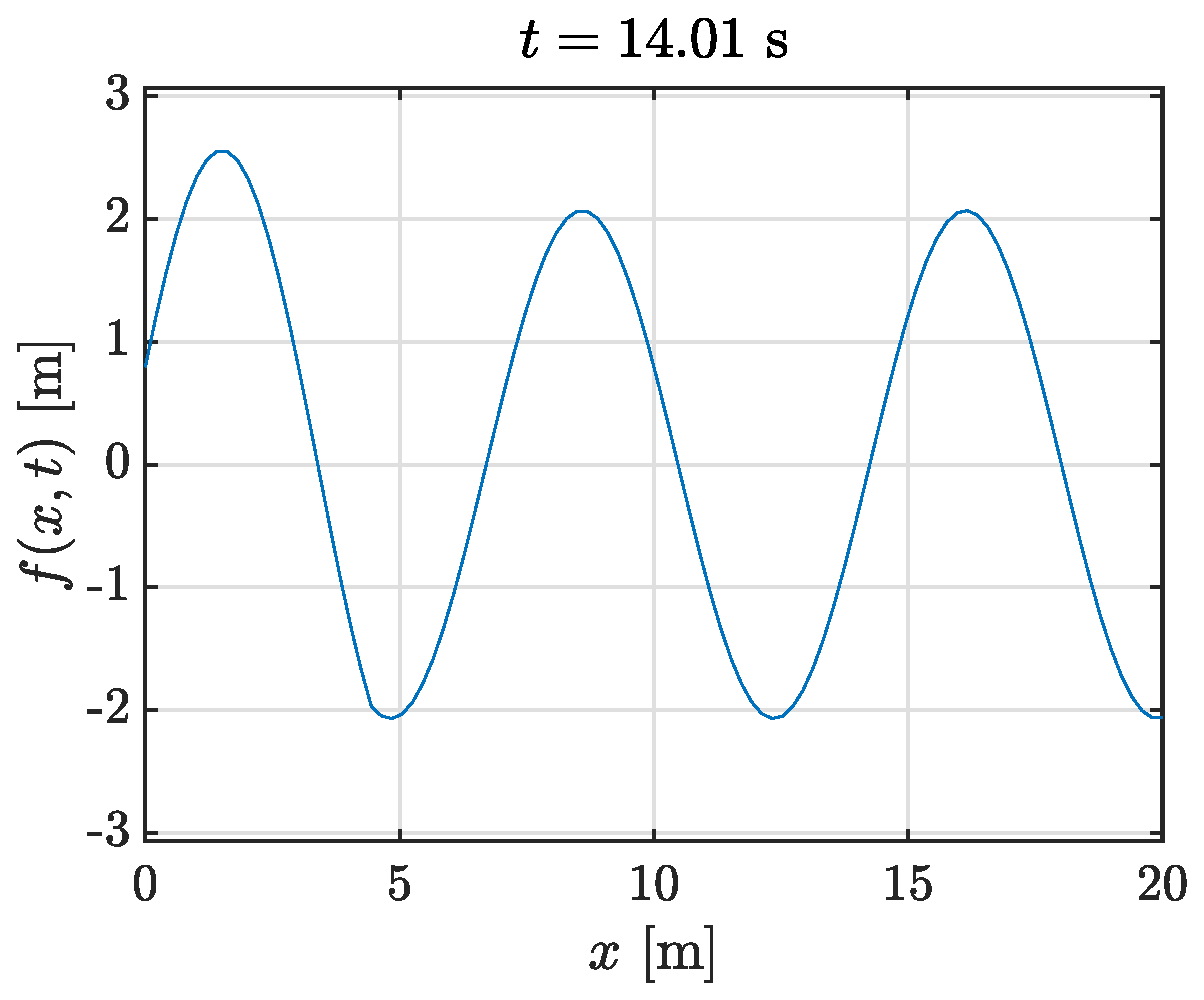
\includegraphics[width=\textwidth]{graphs/ex1flibre.eps}
 \end{subfigure}
 ~
 \begin{subfigure}{0.55\textwidth}
  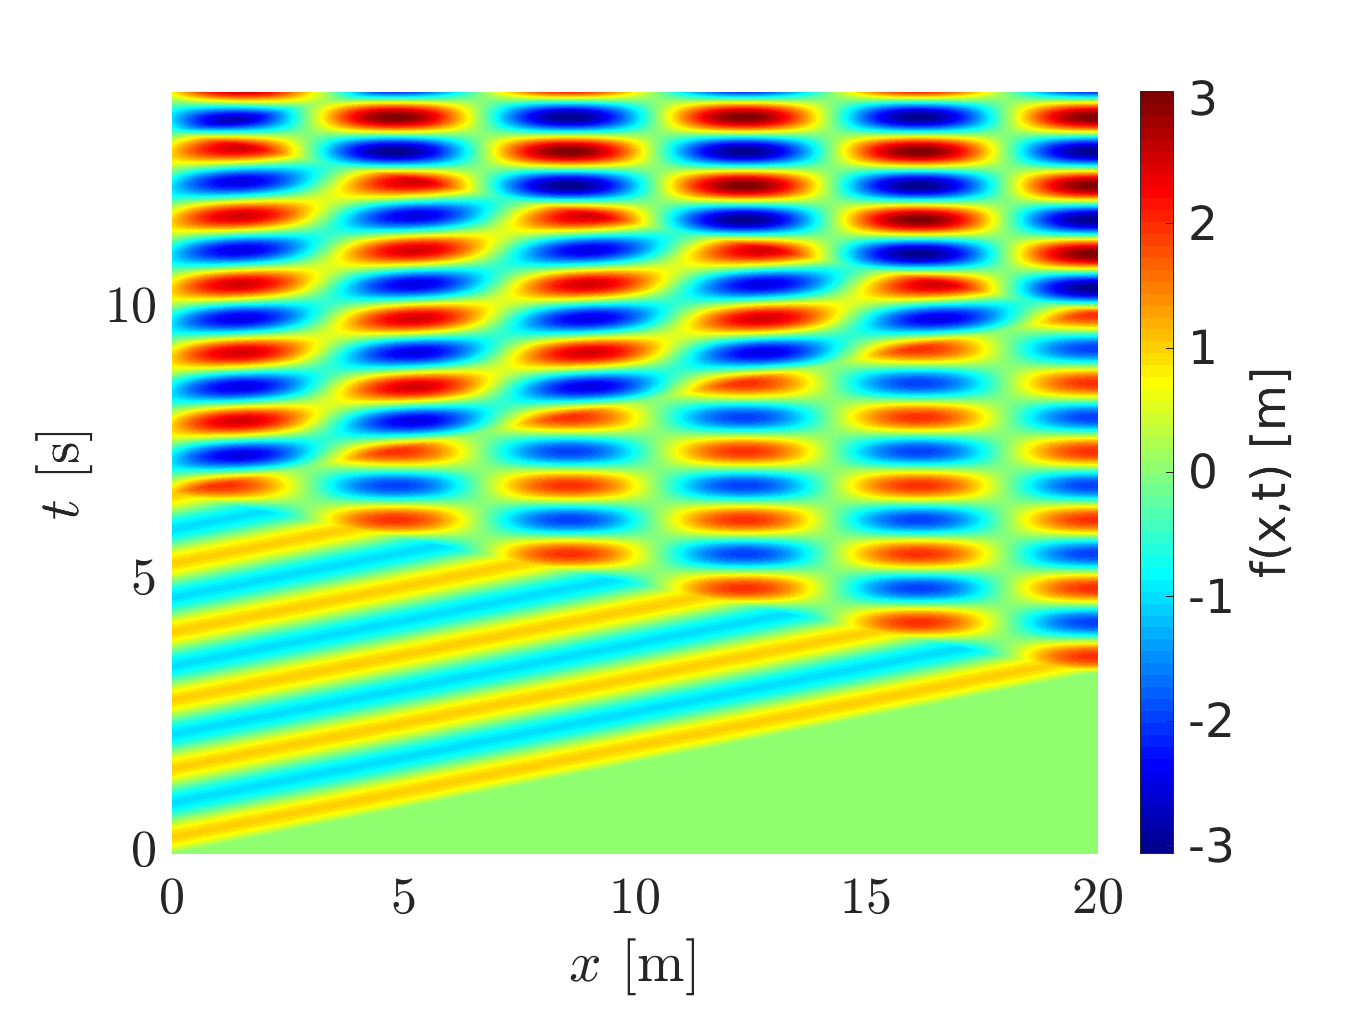
\includegraphics[width=\textwidth]{graphs/ex1xtlibre.eps}
 \end{subfigure}\
 
 \centering
 \begin{subfigure}{0.5\textwidth}
  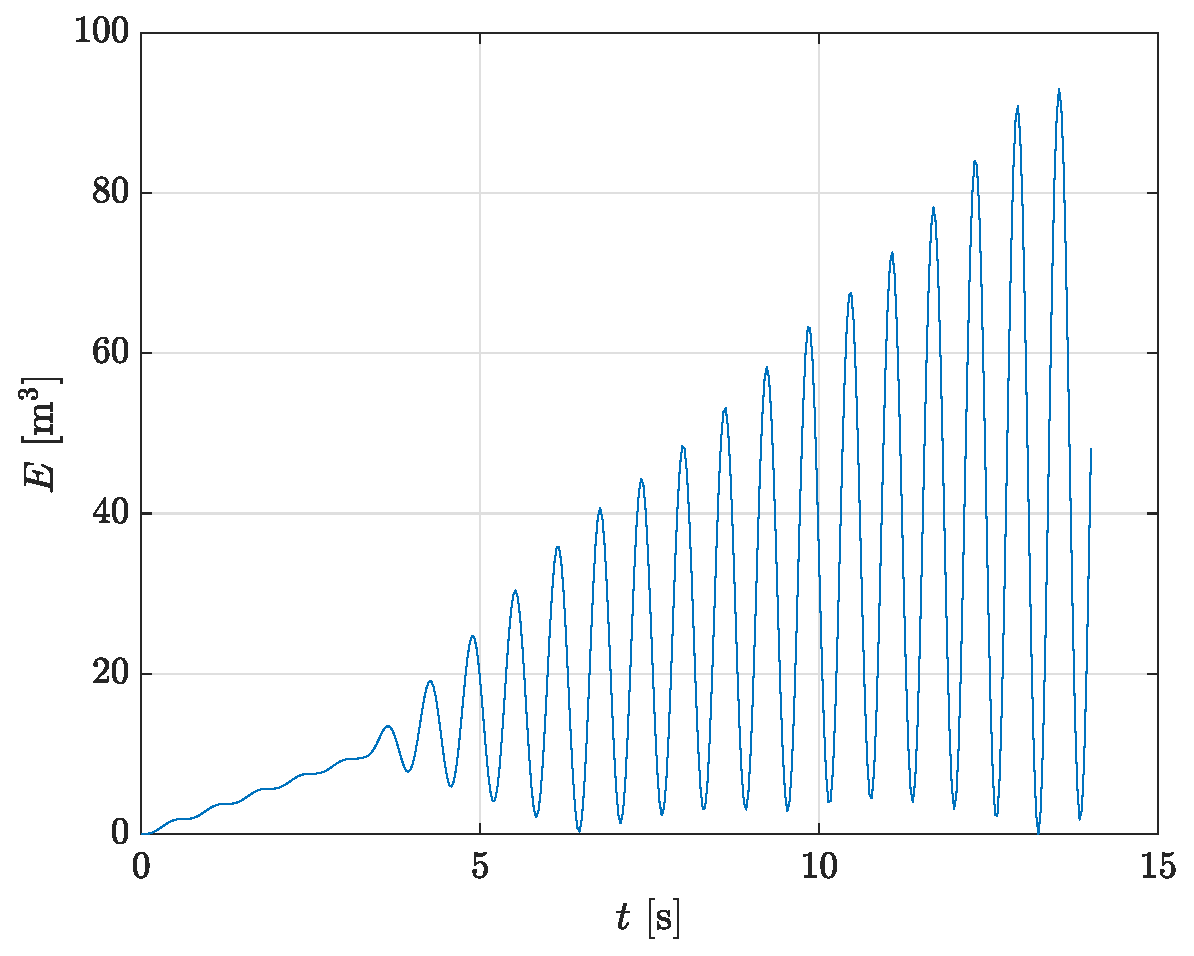
\includegraphics[width=\textwidth]{graphs/ex1Elibre.eps}
 \end{subfigure}

 \caption{Illustration of the border reflection for a the free right border condition}
 \label{fig:ex1fix}
\end{figure}

  % \newpage
  % \begin{thebibliography}{99}
  %
  % \end{thebibliography}

\end{document}
